\documentclass[12pt,oneside,a4paper]{article}
\usepackage[table]{xcolor}
\usepackage{graphicx}
\usepackage{amsmath}
\usepackage{fancyhdr}


\pagestyle{fancy}
\cfoot{\thepage}
\fancyhead{}
\fancyhead[R]{\leftmark}
\renewcommand*\contentsname{Sommaire}

\begin{document}
\title{Report}
\author{Fanny Kalinowski, Julien Molinier, Robin Lambert, Maxime Leras}
\date{25 Mars 2020}
\maketitle
\newpage    
\tableofcontents

\newpage
\pagenumbering{arabic}
\section{Introduction}
\paragraph{}
    Tabu Search is an algorithm created in 1986. It uses a deterministic heuristic on
    local search methods. The goal is to take a potential solution, that's to stay a local optimum,  
    and to check its immediate neighbors in the hope of finding an improved solution.
    \footnote{https://en.wikipedia.org/wiki/Tabu\_search}
\paragraph{}
    The objective of this report is to analyse an implementation of the Tabu Search algorithm through various configurations.
    Then, it will be interesting to discuss on the effects of changing the paramaters values.

\section{Tests without Tabu duration on 10 cities}
\subsection{Run of the algorithm}
\paragraph{}
    First of all we ran the algorithm 10 times for 5, 10 and 100 iterations. The algorithm stops when he found
    the global minimum which is supposed to be 3473km. The results are in the table below :    

\begin{table}[h]
    \centering
    \small
    \begin{tabular}{llll}
      \hline
      \multicolumn{1}{|l|}{\textbf{Run / Nb\_iterations}}& \multicolumn{1}{l|}{\textbf{5}} & \multicolumn{1}{l|}{\textbf{10}} & \multicolumn{1}{l|}{\textbf{100}}\\ \hline
      \multicolumn{1}{|l|}{1} & \multicolumn{1}{l|}{-}  & \multicolumn{1}{l|}{5}  & \multicolumn{1}{l|}{4}  \\ \hline
      \multicolumn{1}{|l|}{2} & \multicolumn{1}{l|}{-}  & \multicolumn{1}{l|}{7}  & \multicolumn{1}{l|}{4}  \\ \hline         
      \multicolumn{1}{|l|}{3} & \multicolumn{1}{l|}{-}  & \multicolumn{1}{l|}{5}  & \multicolumn{1}{l|}{4}  \\ \hline
      \multicolumn{1}{|l|}{4} & \multicolumn{1}{l|}{-}  & \multicolumn{1}{l|}{4}  & \multicolumn{1}{l|}{6}  \\ \hline
      \multicolumn{1}{|l|}{5} & \multicolumn{1}{l|}{-}  & \multicolumn{1}{l|}{6}  & \multicolumn{1}{l|}{4}  \\ \hline
      \multicolumn{1}{|l|}{6} & \multicolumn{1}{l|}{3}  & \multicolumn{1}{l|}{5}  & \multicolumn{1}{l|}{7}  \\ \hline
      \multicolumn{1}{|l|}{7} & \multicolumn{1}{l|}{-}  & \multicolumn{1}{l|}{7}  & \multicolumn{1}{l|}{4}  \\ \hline
      \multicolumn{1}{|l|}{8} & \multicolumn{1}{l|}{-}  & \multicolumn{1}{l|}{7}  & \multicolumn{1}{l|}{4}  \\ \hline
      \multicolumn{1}{|l|}{9} & \multicolumn{1}{l|}{-}  & \multicolumn{1}{l|}{5}  & \multicolumn{1}{l|}{7}  \\ \hline
      \multicolumn{1}{|l|}{10} & \multicolumn{1}{l|}{-}  & \multicolumn{1}{l|}{3}  & \multicolumn{1}{l|}{5}  \\ \hline
    \end{tabular}
    \caption{Number of iteration needed without tabu duration on 10 cities}
  \end{table}

\paragraph{}
    From this table, the computation of the average gives 4.9 on 10 iterations and 4.9 on 100 iterations.
    It means the algorithm needs around 5 iterations to find the global minimum. Thus, it explains why the algorithm
    ended only 1 time when the Nb\_iterations is equal to 5.

\subsection{Convergence}
\paragraph{}
    The values computed in section 2.1 shows that the algorithm needs 5 iterations on average to converge to the
    global minimum. After the algorithm computes the neighbors of this solution but as the previous solution is the
    global minimum the neighbors won't be better. So the global minimum remains the same and the algorithm repeats this step
    again and again until the maximum number of iterations sets before launching. This is why when the maximum is 5 the
    algorithm can't always find the global minimum.

\subsection{Number of solutions and neighbors with 2-opt}
\paragraph{}
    For 10 cities the number of solutions is \textit{9!/2} and for 50 cities it is \textit{49!/2}.
\paragraph{}
    The number of neighbors with 2-opt follows the formula :
    \[\binom{n}{1}\binom{n-3}{1}/2\]
\paragraph{}
    For 10 cities it gives 35 and for 50 cities 1175 neighbors.

\subsection{Algorithm performance}
\paragraph{}
    The number of solutions visited by the algorithm before the convergence is given by the formula
    \textit{Nb\_iterations * Nb\_neighbors}. So with 10 cities if the algorithm finds the solution at the 
    iteration 4 it means that 40 solutions were visited. Compared to the 9! possible ones the algorithm tries only 1
    out of 10000 solutions; this is pretty good.
\newpage

\section{Tests without Tabu duration on 50 cities}
\subsection{Run of the algorithm}
\begin{table}[h]
    \centering
    \small
    \begin{tabular}{llll}
      \hline
      \multicolumn{1}{|l|}{\textbf{Run / Nb\_iterations}}& \multicolumn{1}{l|}{\textbf{10}} & \multicolumn{1}{l|}{\textbf{100}} & \multicolumn{1}{l|}{\textbf{1000}}\\ \hline
      \multicolumn{1}{|l|}{1} & \multicolumn{1}{l|}{-}  & \multicolumn{1}{l|}{44}  & \multicolumn{1}{l|}{50}  \\ \hline
      \multicolumn{1}{|l|}{2} & \multicolumn{1}{l|}{-}  & \multicolumn{1}{l|}{44}  & \multicolumn{1}{l|}{47}  \\ \hline         
      \multicolumn{1}{|l|}{3} & \multicolumn{1}{l|}{-}  & \multicolumn{1}{l|}{48}  & \multicolumn{1}{l|}{43}  \\ \hline
      \multicolumn{1}{|l|}{4} & \multicolumn{1}{l|}{-}  & \multicolumn{1}{l|}{48}  & \multicolumn{1}{l|}{46}  \\ \hline
      \multicolumn{1}{|l|}{5} & \multicolumn{1}{l|}{-}  & \multicolumn{1}{l|}{40}  & \multicolumn{1}{l|}{44}  \\ \hline
      \multicolumn{1}{|l|}{6} & \multicolumn{1}{l|}{-}  & \multicolumn{1}{l|}{42}  & \multicolumn{1}{l|}{44}  \\ \hline
      \multicolumn{1}{|l|}{7} & \multicolumn{1}{l|}{-}  & \multicolumn{1}{l|}{44}  & \multicolumn{1}{l|}{47}  \\ \hline
      \multicolumn{1}{|l|}{8} & \multicolumn{1}{l|}{-}  & \multicolumn{1}{l|}{43}  & \multicolumn{1}{l|}{42}  \\ \hline
      \multicolumn{1}{|l|}{9} & \multicolumn{1}{l|}{-}  & \multicolumn{1}{l|}{42}  & \multicolumn{1}{l|}{43}  \\ \hline
      \multicolumn{1}{|l|}{10} & \multicolumn{1}{l|}{-}  & \multicolumn{1}{l|}{44}  & \multicolumn{1}{l|}{47}  \\ \hline
    \end{tabular}
    \caption{Number of iteration needed without tabu duration on 50 cities}
  \end{table}
\paragraph{}
    For 10 iterations, the algorithm never found the global minimum. On average, the global minimum is found at the 43.9th
    for 100 iterations. For 1000 iterations, the global minimum is found at the 45.3th iteration.

\subsection{Convergence}
\paragraph{}
    The algorithm needs around 43.9 iterations to converge for Nb\_iterations equal to 100 iterations, and 45.3 iterations to converge for Nb\_iterations equal to 1000 iterations. 
\paragraph{}
    Once the algorithm have found the global minimum, it doesn't explore other paths. In the following iterations, the value of the kilometers is still blocked on the global minimum. 
    According to the algorithm, the global minima is the best solution until yet, so there is no need to explore the neighborhood around the top.  
    This is due to the Duration\_tabou which is equal to 0. This means that the number of solution that have been explored successively are not kept in memory. 
    Thus, the same points are explored several times. Consequently, the local minima is not going to change.

\newpage
\subsection{Solutions visited before the convergence}
\paragraph{}
    The algorithm starts to converge once it has found a local minima.
    So, in order to know the number of solutions visited before its convergence we need to count all the solutions 
    that have been explored before the finding of the local minima. 
    In the first run, with Nb\_iterations equal to 100, \textit{Iteration\_of\_best\_soultion*1175} solutions have been explored before the finding of the local minima. 
    So, for each of the iterations, the best solution is displayed. It’s the result of the exploration of all the 1175 neighbors.

    \begin{table}[h]
        \centering
        \small
        \begin{tabular}{llll}
          \hline
          \multicolumn{1}{|l|}{\textbf{Run / Nb\_iterations}}& \multicolumn{1}{l|}{\textbf{10}} & \multicolumn{1}{l|}{\textbf{100}} & \multicolumn{1}{l|}{\textbf{1000}}\\ \hline
          \multicolumn{1}{|l|}{1} & \multicolumn{1}{l|}{-}  & \multicolumn{1}{l|}{43}  & \multicolumn{1}{l|}{49}  \\ \hline
          \multicolumn{1}{|l|}{2} & \multicolumn{1}{l|}{-}  & \multicolumn{1}{l|}{43}  & \multicolumn{1}{l|}{46}  \\ \hline         
          \multicolumn{1}{|l|}{3} & \multicolumn{1}{l|}{-}  & \multicolumn{1}{l|}{47}  & \multicolumn{1}{l|}{42}  \\ \hline
          \multicolumn{1}{|l|}{4} & \multicolumn{1}{l|}{-}  & \multicolumn{1}{l|}{47}  & \multicolumn{1}{l|}{45}  \\ \hline
          \multicolumn{1}{|l|}{5} & \multicolumn{1}{l|}{-}  & \multicolumn{1}{l|}{39}  & \multicolumn{1}{l|}{43}  \\ \hline
          \multicolumn{1}{|l|}{6} & \multicolumn{1}{l|}{-}  & \multicolumn{1}{l|}{41}  & \multicolumn{1}{l|}{43}  \\ \hline
          \multicolumn{1}{|l|}{7} & \multicolumn{1}{l|}{-}  & \multicolumn{1}{l|}{43}  & \multicolumn{1}{l|}{46}  \\ \hline
          \multicolumn{1}{|l|}{8} & \multicolumn{1}{l|}{-}  & \multicolumn{1}{l|}{42}  & \multicolumn{1}{l|}{41}  \\ \hline
          \multicolumn{1}{|l|}{9} & \multicolumn{1}{l|}{-}  & \multicolumn{1}{l|}{41}  & \multicolumn{1}{l|}{42}  \\ \hline
          \multicolumn{1}{|l|}{10} & \multicolumn{1}{l|}{-}  & \multicolumn{1}{l|}{41}  & \multicolumn{1}{l|}{46}  \\ \hline
        \end{tabular}
        \caption{Number of iterations before the finding of the best solution without Duration\_tabou on 50 cities}
      \end{table}

      \begin{table}[h]
        \centering
        \small
        \begin{tabular}{llll}
          \hline
          \multicolumn{1}{|l|}{\textbf{Run / Nb\_iterations}}& \multicolumn{1}{l|}{\textbf{10}} & \multicolumn{1}{l|}{\textbf{100}} & \multicolumn{1}{l|}{\textbf{1000}}\\ \hline
          \multicolumn{1}{|l|}{1} & \multicolumn{1}{l|}{-}  & \multicolumn{1}{l|}{50525}  & \multicolumn{1}{l|}{57575}  \\ \hline
          \multicolumn{1}{|l|}{2} & \multicolumn{1}{l|}{-}  & \multicolumn{1}{l|}{50525}  & \multicolumn{1}{l|}{54060}  \\ \hline         
          \multicolumn{1}{|l|}{3} & \multicolumn{1}{l|}{-}  & \multicolumn{1}{l|}{55225}  & \multicolumn{1}{l|}{49350}  \\ \hline
          \multicolumn{1}{|l|}{4} & \multicolumn{1}{l|}{-}  & \multicolumn{1}{l|}{55225}  & \multicolumn{1}{l|}{52875}  \\ \hline
          \multicolumn{1}{|l|}{5} & \multicolumn{1}{l|}{-}  & \multicolumn{1}{l|}{45825}  & \multicolumn{1}{l|}{50525}  \\ \hline
          \multicolumn{1}{|l|}{6} & \multicolumn{1}{l|}{-}  & \multicolumn{1}{l|}{48175}  & \multicolumn{1}{l|}{50525}  \\ \hline
          \multicolumn{1}{|l|}{7} & \multicolumn{1}{l|}{-}  & \multicolumn{1}{l|}{50525}  & \multicolumn{1}{l|}{54060}  \\ \hline
          \multicolumn{1}{|l|}{8} & \multicolumn{1}{l|}{-}  & \multicolumn{1}{l|}{49350}  & \multicolumn{1}{l|}{48175}  \\ \hline
          \multicolumn{1}{|l|}{9} & \multicolumn{1}{l|}{-}  & \multicolumn{1}{l|}{48175}  & \multicolumn{1}{l|}{49350}  \\ \hline
          \multicolumn{1}{|l|}{10} & \multicolumn{1}{l|}{-}  & \multicolumn{1}{l|}{48175}  & \multicolumn{1}{l|}{54060}  \\ \hline
        \end{tabular}
        \caption{Number of solutions visited before the convergence without Duration\_tabou on 50 cities}
      \end{table}

\paragraph{}
    On average, 50172.5 solutions have been explored before finding the local minima for Nb\_iterations equal to 100, against 52055.5 explored solutions for Nb\_iterations equal to 1000.
    The two runs show that the local minima is found between the 42.7th and the 44.3th iteration. 

    This is logical, since the Duration\_tabou is equal to 0 in the two runs. 
    Increasing the number of iterations is interesting if the value of the Duration\_tabou changes. In fact, it will allow the algorithm not to go through the same path 
    and to have more time (thanks to the iterations) to explore.
    If the value of the Duration\_tabou doesn’t change, once the algorithm have found the local minima, it will stop to converge to it, no matters the number of iterations. 
    So here, the number of iterations does not influence the local minima.

    On 100 iterations, the local minima is found at the 43th iteration. It results of a convergence. In the 57 following iterations, the algorithm is blocked to this local minima. That’s to say that 
    during 57 iterations there is not relevant information, as the local minima is not going to change. 
    On 1000 iterations, the algorithm converges to the local minima. It's found at the 44th iteration. So, the algorithm is blocked in the following 956 iterations, meaning that during 
    956 iterations there is not relevant information. The neighbors are not visited since there are less interesting than the local minima.

    Since the time loss is less important on 100 iterations than on 1000 iterations, the one can say that running the algorithm on 100 iterations allows to gain performance.
    

\section{Tests with Tabu duration}
\subsection{Run of the algorithm}
The algorithm was run 10 times for Nb\_iterations equal to 1000.
\begin{table}[h]
    \centering
    \small
    \begin{tabular}{llll}
      \hline
      \multicolumn{1}{|l|}{\textbf{Run}}& \multicolumn{1}{l|}{\textbf{Best solution in km}}& \multicolumn{1}{l|}{\textbf{Nb\_local minima visited}}& \multicolumn{1}{l|}{\textbf{Nb\_BetterSolution}}\\ \hline
      \multicolumn{1}{|l|}{1} & \multicolumn{1}{l|}{5691}  & \multicolumn{1}{l|}{265} & \multicolumn{1}{l|}{43}  \\ \hline
      \multicolumn{1}{|l|}{2} & \multicolumn{1}{l|}{5691}  & \multicolumn{1}{l|}{300} & \multicolumn{1}{l|}{54}  \\ \hline         
      \multicolumn{1}{|l|}{3} & \multicolumn{1}{l|}{5644}  & \multicolumn{1}{l|}{294}  & \multicolumn{1}{l|}{47}  \\ \hline
      \multicolumn{1}{|l|}{4} & \multicolumn{1}{l|}{5644}  & \multicolumn{1}{l|}{226}  & \multicolumn{1}{l|}{49}  \\ \hline
      \multicolumn{1}{|l|}{5} & \multicolumn{1}{l|}{5771}  & \multicolumn{1}{l|}{271}  & \multicolumn{1}{l|}{48}  \\ \hline
      \multicolumn{1}{|l|}{6} & \multicolumn{1}{l|}{5644}  & \multicolumn{1}{l|}{271}  & \multicolumn{1}{l|}{47}  \\ \hline
      \multicolumn{1}{|l|}{7} & \multicolumn{1}{l|}{5798}  & \multicolumn{1}{l|}{242}  & \multicolumn{1}{l|}{49}  \\ \hline
      \multicolumn{1}{|l|}{8} & \multicolumn{1}{l|}{5770}  & \multicolumn{1}{l|}{276} & \multicolumn{1}{l|}{62}  \\ \hline
      \multicolumn{1}{|l|}{9} & \multicolumn{1}{l|}{5644}  & \multicolumn{1}{l|}{300} & \multicolumn{1}{l|}{48}  \\ \hline
      \multicolumn{1}{|l|}{10} & \multicolumn{1}{l|}{5720}  & \multicolumn{1}{l|}{216} & \multicolumn{1}{l|}{59}  \\ \hline
    \end{tabular}
    \caption{Number of local minima visited with tabu duration on 50 cities}
  \end{table}

\subsection{Improving the best solution}
\paragraph{}
    On average, the best solution is improved 50.6 times in a run. This is mostly due to the first
    descent to the first found local minima but if we count the number of local minimum that improve
    the previous local minima, we have an average of 3 improvements in a run.

\subsection{Local minima}
\paragraph{}
    On average, 266 local minima are visited by the algorithm. 
    Duration\_tabou is the number of solutions that have been explored successively. They are kept in memory like a path. So, the solutions belonging to the path could
    not be explored anymore. The one can see that the path allows the algorithm to escape from the mountains. It goes to a local optimum, escapes and then goes to another one. 
    After having visited all the local minima, the algorithm can find the major top, so the best solution. Consequently, the algorithm doesn’t converge because the solution 
    moves from one local optima to another one. New local minima can be explored and the global minima can be updated. Introducing the tabu duration allows to use properly
    the algorithm. First, the Tabu search for the best neighbor up to the local optimum. 
    After being on the top, it explores around the top in order to find the best neighbor. So, the metric Duration\_tabou allows to search other neighbors by memorizing and 
    excluding the previous paths.  This is why new local optima are found.
    After going down this area, the algorithm jump to another local optimum and explore new paths.
    Doing this way, the algorithm moves from one area to another one. At the end, the major top is the result of a complete exploration. 

    In the section B, with the following configuration ./algo\_tabou  1000 0 50 distances\_entre\_villes\_50.txt the best solution is on average  5891.7 km.

    In this section, with the following configuration ./algo\_tabou  1000 10 50 distances\_entre\_villes\_50.txt
    the best solution is on average 5701.7 km.

    So, introducing the Duration\_tabou allows the algorithm to gain in performance in terms of space because new mountains with new local minima are explored. At the end 
    of the exploration, the less local minima can be considered as the major top, thus as the best solution.
    With the Duration\_tabou equals to zero, only the local optimum of one area is explored. If we’re lucky, the best solution is contained in this unique area. But in most cases,
    the major local minima is contained in another mountain. So what the algorithm considers as the best solution is probably the wrong one.

    Nevertheless, 5701.7 km may not be the best solution of all the area. In this configuration, only 10 solutions are registered and belong to the path. It’s possible that
    the solutions who do not belong the path have been explored more than once. We have to change the value of the Duration\_tabou increase, to see the effects of 
    expanding the path.

\newpage
\section{Variation in Tabu duration}
\subsection{Explanation on the code}
\paragraph{}
    The Tabu list is coded so that it can be able to store for a couple of two cities if an switch move for all cities between them is Tabu or not. Here's an example of this move bewteen the cities A and B :
    \newline


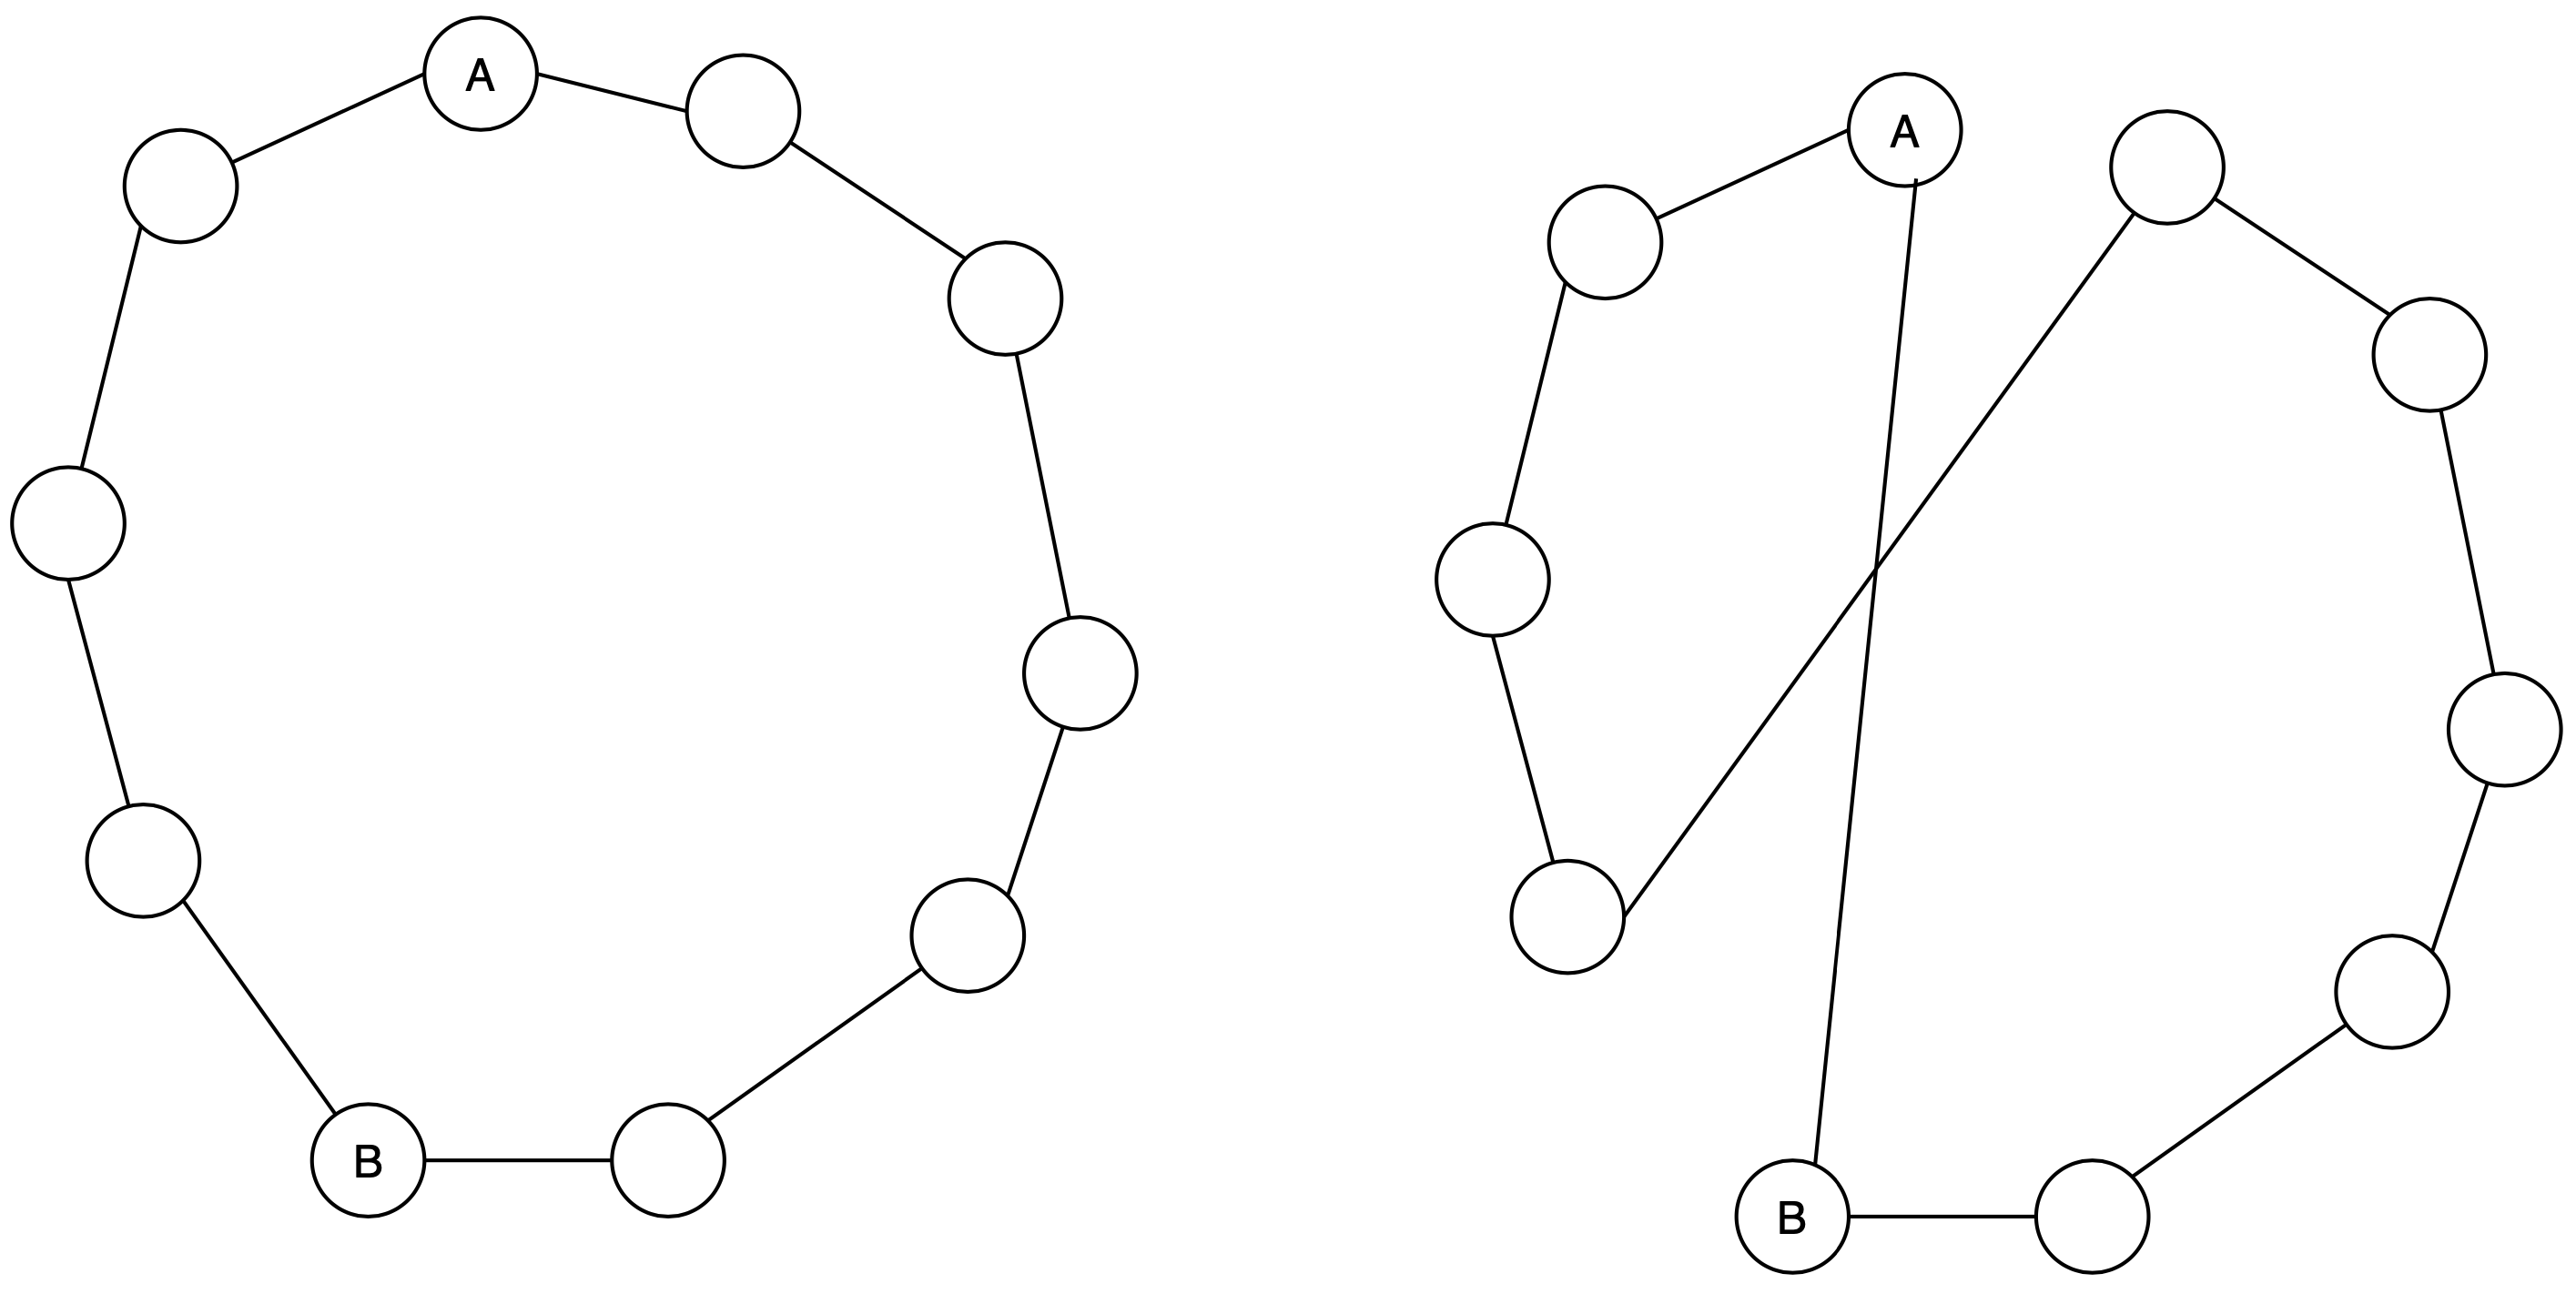
\includegraphics[width=0.8\textwidth]{move.png}\\
\paragraph{}
    Such a move is considered as "tabu" if it has already been done before.
    However, the code will not remember a move after a specific number of iterations : this is the tabu duration. Added to the current iteration number, its value is stored inside the tabu list for a couple of two cities.
    By comparing the stored value to the current iteration, the algorithm can determine if the move is tabu or not ('-1' is stored for each couple before exploring any solution, so the first move cannot be tabu).
    There's also another list in the code which stores all tabu solutions, instead of the moves. This list could have been used too.
\paragraph{}
    The algorithm explores all possible moves (between each cities) for a given solution : this is the neighborhood. The best solution which resulted from a switch move which is not tabu is now defined as the current one.
\paragraph{}
    The interesting thing is that the tabu list avoid the algorithm to be stuck in a local minimum. Because it chooses the best solution amongs the non visited neighboors, it can go for a solution which isn't necesserly improving the result.
    If the tabu duration is long enough, it can easily get out of local minimum. However, choosing a too important value is not a good idea, because it can be completely surrounded by already visited solutions, or surround the best solution and be stuck again.
    So technically, it is possible to chose a tabu duration as long as the number of iterations, but of course it is not a good practice to do so.



\subsection{Run of the algorithm}
  The algorithm was run 5 times for Nb\_iterations equal to 1000.
\begin{table}[h]
    \centering
    \small
    \begin{tabular}{llllll}
      \hline
      \multicolumn{1}{|l|}{\textbf{Run / Duration\_tabou}}& \multicolumn{1}{l|}{\textbf{20}} & \multicolumn{1}{l|}{\textbf{50}} & \multicolumn{1}{l|}{\textbf{80}} & \multicolumn{1}{l|}{\textbf{100}} & \multicolumn{1}{l|}{\textbf{1000}}\\ \hline
      \multicolumn{1}{|l|}{1} & \multicolumn{1}{l|}{250}  & \multicolumn{1}{l|}{209}  & \multicolumn{1}{l|}{218}   & \multicolumn{1}{l|}{220}  & \multicolumn{1}{l|}{286} \\ \hline
      \multicolumn{1}{|l|}{2} & \multicolumn{1}{l|}{239}  & \multicolumn{1}{l|}{213}  & \multicolumn{1}{l|}{198}  & \multicolumn{1}{l|}{208}  & \multicolumn{1}{l|}{270} \\ \hline         
      \multicolumn{1}{|l|}{3} & \multicolumn{1}{l|}{228}  & \multicolumn{1}{l|}{219}  & \multicolumn{1}{l|}{207}  & \multicolumn{1}{l|}{243}  & \multicolumn{1}{l|}{274} \\ \hline
      \multicolumn{1}{|l|}{4} & \multicolumn{1}{l|}{253}  & \multicolumn{1}{l|}{200}  & \multicolumn{1}{l|}{209}   & \multicolumn{1}{l|}{235}  & \multicolumn{1}{l|}{281}\\ \hline
      \multicolumn{1}{|l|}{5} & \multicolumn{1}{l|}{231}  & \multicolumn{1}{l|}{229}  & \multicolumn{1}{l|}{216}   & \multicolumn{1}{l|}{223}  & \multicolumn{1}{l|}{273}\\ \hline
    \end{tabular}
    \caption{Number of local minima visited with various Duration\_tabou on 50 cities}
  \end{table}
  \begin{table}[h]
    \centering
    \small
    \begin{tabular}{llllll}
      \hline
      \multicolumn{1}{|l|}{\textbf{Run / Duration\_tabou}}& \multicolumn{1}{l|}{\textbf{20}} & \multicolumn{1}{l|}{\textbf{50}} & \multicolumn{1}{l|}{\textbf{80}} & \multicolumn{1}{l|}{\textbf{100}} & \multicolumn{1}{l|}{\textbf{1000}}\\ \hline
      \multicolumn{1}{|l|}{1} & \multicolumn{1}{l|}{5649}  & \multicolumn{1}{l|}{5649}  & \multicolumn{1}{l|}{5746}   & \multicolumn{1}{l|}{5698}  & \multicolumn{1}{l|}{5867} \\ \hline
      \multicolumn{1}{|l|}{2} & \multicolumn{1}{l|}{5649}  & \multicolumn{1}{l|}{5775}  & \multicolumn{1}{l|}{5706}  & \multicolumn{1}{l|}{5780}  & \multicolumn{1}{l|}{5715} \\ \hline         
      \multicolumn{1}{|l|}{3} & \multicolumn{1}{l|}{5799}  & \multicolumn{1}{l|}{5649}  & \multicolumn{1}{l|}{5649}  & \multicolumn{1}{l|}{5711}  & \multicolumn{1}{l|}{5803} \\ \hline
      \multicolumn{1}{|l|}{4} & \multicolumn{1}{l|}{5649}  & \multicolumn{1}{l|}{5809}  & \multicolumn{1}{l|}{5716}   & \multicolumn{1}{l|}{5692}  & \multicolumn{1}{l|}{5764}\\ \hline
      \multicolumn{1}{|l|}{5} & \multicolumn{1}{l|}{5649}  & \multicolumn{1}{l|}{5682}  & \multicolumn{1}{l|}{5661}   & \multicolumn{1}{l|}{5691}  & \multicolumn{1}{l|}{5716}\\ \hline
    \end{tabular}
    \caption{Best solutions with various Duration\_tabou on 50 cities}
  \end{table}

\subsection{Improving the best solution}
  A compléter
\subsection{Local minima}
\begin{table}[h]
    \centering
    \small
    \begin{tabular}{llllll}
      \hline
      \multicolumn{1}{|l|}{\textbf{Duration\_tabou}}& \multicolumn{1}{l|}{\textbf{20}} & \multicolumn{1}{l|}{\textbf{50}} & \multicolumn{1}{l|}{\textbf{80}} & \multicolumn{1}{l|}{\textbf{100}} & \multicolumn{1}{l|}{\textbf{1000}}\\ \hline
      \multicolumn{1}{|l|}{local minima } & \multicolumn{1}{l|}{120.1}  & \multicolumn{1}{l|}{107}  & \multicolumn{1}{l|}{104.8}   & \multicolumn{1}{l|}{112.7}  & \multicolumn{1}{l|}{138.4} \\ \hline
    \end{tabular}
    \caption{Average of local minima visited with various Duration\_tabou on 50 cities}
  \end{table}
\paragraph{}
A completer : convergence + conclusions

\newpage
\subsection{Parameters settings recommanded}
\begin{table}[h]
    \centering
    \small
    \begin{tabular}{llllll}
      \hline
      \multicolumn{1}{|l|}{\textbf{Duration\_tabou}}& \multicolumn{1}{l|}{\textbf{20}} & \multicolumn{1}{l|}{\textbf{50}} & \multicolumn{1}{l|}{\textbf{80}} & \multicolumn{1}{l|}{\textbf{100}} & \multicolumn{1}{l|}{\textbf{1000}}\\ \hline
      \multicolumn{1}{|l|}{best solution in km } & \multicolumn{1}{l|}{2839.5}  & \multicolumn{1}{l|}{2856.4}  & \multicolumn{1}{l|}{2847.8}   & \multicolumn{1}{l|}{2857.2}  & \multicolumn{1}{l|}{2856.5} \\ \hline
    \end{tabular}
    \caption{Average of best solutions obtained with various Duration\_tabou on 50 cities}
  \end{table}
\paragraph{}
    In the section C, with the following configuration ./algo\_tabou  1000 10 50 distances\_entre\_villes\_50.txt the best solution is 5701.7 km. 
    If we double the Duration\_tabou, the best solution is reduced by two :  2839.5 km.
    So, the solution is even more better with a big Duration\_tabou. 

    We can observe that increasing the Duration\_tabou more than 20 has no good effects on the best solution because it becomes bigger and bigger. 
    But it’s still less than Duration\_tabou= 10. 

    A completer

\subsection{Infinite value for the Tabu duration}
\paragraph{}
  The Tabu Duration prohibits to reuse the move for a number of iterations. This is why the number must be set according to the number of variables 
  and possible values for the variables. In fact if this number is to big all moves will be prohibited and the algorithm blocked.
\section{Conclusion}
\paragraph{}

\end{document}